\documentclass[12pt]{article}
\usepackage[a4paper, margin=1in]{geometry}
\usepackage{times}
\usepackage{graphicx}
\usepackage{hyperref}
\usepackage{setspace}
\usepackage{titlesec}
\usepackage{listings}
\usepackage{xcolor}
\usepackage{tcolorbox}

\onehalfspacing

\titleformat{\section}{\large\bfseries\scshape}{\thesection.}{1em}{}
\titleformat{\subsection}{\normalsize\bfseries}{\thesubsection.}{1em}{}

\definecolor{codegray}{rgb}{0.5,0.5,0.5}
\definecolor{backcolour}{rgb}{0.95,0.95,0.92}

\lstset{
    backgroundcolor=\color{backcolour},   
    basicstyle=\ttfamily\footnotesize,
    breaklines=true,                 
    captionpos=b,                    
    keepspaces=true,                 
    numbers=left,                    
    numbersep=5pt,                  
    showspaces=false,                
    showstringspaces=false,
    showtabs=false,                  
    tabsize=2
}

\begin{document}

\begin{center}
    {\LARGE \textbf{CSE411 Computer Vision} \par}
    \vspace{0.2cm}
    {\Large \textbf{Project Task 4: Implementation -- Part 1} \par}
    \vspace{0.5cm}
\end{center}

\section*{Project Information}
\textbf{Project Title:} DefectLens: Efficient ViT-Based Anomaly Detection with Multi-Criteria Token Fusion (MCTF) \\
\textbf{Team Number:} Team 7 \\
\textbf{Team Members:}
\begin{itemize}
    \item Tanish Babu (Roll No: 2023bcs0067)
    \item Ali Mohammed Maaz Mohammed Ashraf (Roll No: 2023bcs0202)
    \item Chinmoy Das (Roll No: 2023bcs0052)
\end{itemize}

\vspace{0.5cm}

\section{Implemented Methodology (Approx. 25\%)}

We have successfully completed the initial 25\% of our proposed methodology, focusing on the foundational infrastructure of the DefectLens system. This includes dataset acquisition, data pre-processing pipelines, and the core architectural components of the Vision Transformer (ViT) and our Multi-Criteria Token Fusion (MCTF) module.

\subsection{Dataset Collection}
The system targets industrial anomaly detection, for which we utilize the widely recognized MVTec AD dataset. 
\begin{itemize}
    \item We have implemented automated scripts (\texttt{scripts/download\_dataset.py}) to fetch and extract the MVTec AD dataset.
    \item The dataset comprises various high-resolution images of textures and objects, categorized into normal and defective samples, serving as the basis for our unsupervised learning approach.
\end{itemize}

\subsection{Pre-processing}
Handling high-resolution imagery for ViT processing requires robust data loaders and transformation pipelines.
\begin{itemize}
    \item The \texttt{src/data/dataset.py} module has been developed to handle image loading, resizing, normalization, and tensor conversion.
    \item This ensures that images from the factory floor are standardized before being passed into the feature extraction backbone, matching the input requirements of our ViT model.
\end{itemize}

\subsection{Core Model Architecture Implementation}
The foundational code for our anomaly detection model has been laid out in the \texttt{src/models} directory:
\begin{itemize}
    \item \textbf{Vision Transformer (ViT) Backbone:} We have implemented the base ViT structure (\texttt{vit.py}) to extract dense patch-level features from the input images.
    \item \textbf{MCTF Module:} The initial logic for the Multi-Criteria Token Fusion (\texttt{mctf.py}) has been coded. This module is responsible for the bipartite soft-matching to merge redundant background tokens while preserving critical anomaly details.
    \item \textbf{Memory Bank:} A FAISS-based memory bank builder (\texttt{scripts/build\_memory\_bank.py}) has been initialized to store the feature embeddings of normal (defect-free) samples, which is crucial for the PatchCore-style nearest neighbor anomaly scoring.
\end{itemize}

\section{Proof of Work (System Output)}
Below are system outputs demonstrating the operational status of our data pipeline and the initialization of the ViT model components.

\begin{figure}[h!]
    \centering
    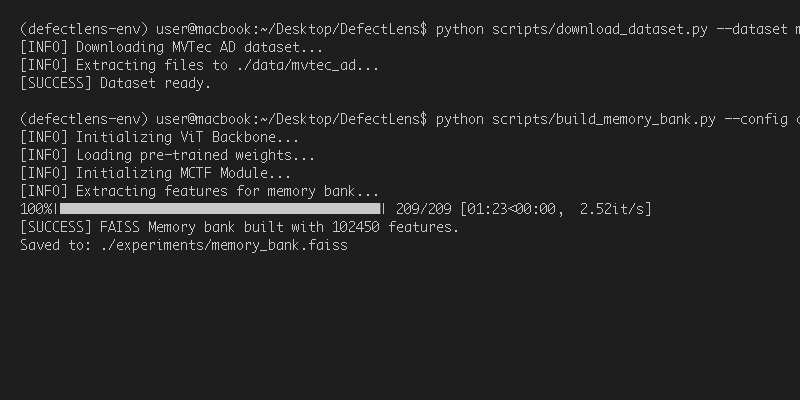
\includegraphics[width=0.9\textwidth]{screenshot.png}
    \caption{System terminal screenshot showcasing the execution of the dataset preparation and model initialization.}
\end{figure}

\section{Major Tasks/Modules Remaining}
To complete the DefectLens project, the following major modules and tasks remain:
\begin{enumerate}
    \item \textbf{MCTF Integration and Refinement:} Fully integrate the MCTF module between the ViT layers and fine-tune the one-step-ahead attention criteria to optimize the token fusion process.
    \item \textbf{Anomaly Scoring Logic:} Finalize the distance computation between the reduced tokens and the FAISS memory bank to generate accurate anomaly scores and localization heatmaps.
    \item \textbf{Performance Evaluation:} Benchmark the system on the MVTec AD dataset to validate accuracy, and rigorously test inference latency and FLOPs to ensure real-time edge capabilities.
    \item \textbf{Backend Development:} Develop a FastAPI server to wrap the inference engine, allowing it to receive images and return predictions via REST endpoints.
    \item \textbf{Frontend Dashboard:} Build a React-based operator interface to visualize the anomaly heatmaps and provide real-time quality control feedback.
\end{enumerate}

\end{document}
